%=============================================================
%  WPOS / UnB — Artigo V1 (revisão crítica da V0)
%  Template: IEEEtran (conferência, 2 colunas). Máx. 4 páginas.
%
%  Compilar: pdflatex v1.tex  (2x, por causa das referências)
%  Requer: IEEEtran.cls (TeX Live / Overleaf) e forest_postura_piloto.png
%          (nesta pasta): a figura do piloto, congelada — a da execução do
%          estudo muda conforme a coleta avança. No compilador online, suba
%          este arquivo junto com o .tex.
%
%  Mudanças V0 -> V1 (ver ficha de revisão crítica):
%   (1) Lacuna: contraste explícito com Germani & Spitale (novidade concreta).
%   (2) Medidas: justificada a escolha do Jev sobre léxico/NLI (validade).
%   (3) Referências: checagem bidirecional (todas citadas / todas com entrada)
%       e padronização de formato.
%
%  Estrutura pensada para sobreviver ao estudo completo: ao fechar a
%  coleta (3 modelos, 20 propostas), substituir apenas os resultados no
%  resumo, as tabelas tab:p1 e tab:p2 e a figura fig:postura — marcados
%  com "% COMPLETO:".
%  Números conferidos com o repositório LucasMABF/Compex, execução
%  results/runs/2026-10-12_003953_estudo (piloto, Claude Sonnet 5.5),
%  e com PLANO_ANALISE.md (pré-registro).
%=============================================================
\documentclass[conference]{IEEEtran}

\usepackage[utf8]{inputenc}
\usepackage[T1]{fontenc}
\usepackage[brazil]{babel}
\usepackage{amsmath,amssymb}
\usepackage{booktabs}
\usepackage{graphicx}
\usepackage{tikz}
\usetikzlibrary{arrows.meta, positioning}
\usepackage{url}

\begin{document}

\title{Robustez do \textit{guardrail} de neutralidade de LLMs à autoria
atribuída\\
\large\textnormal{(versão preliminar --- protocolo e piloto)}}

\author{%
\IEEEauthorblockN{Caio Fernando, Davi Bragança, Eric Wu, Lucas Mendes}
\IEEEauthorblockA{Departamento de Ciência da Computação\\
Universidade de Brasília (UnB), Brasília, Brasil}}

\maketitle

\begin{abstract}
Modelos de linguagem de grande escala (LLMs) são treinados para manter um tom
neutro ao tratar de temas políticos controversos. Investigamos se essa
neutralidade é \emph{invariante à autoria atribuída} a uma proposta: a mesma
proposta é submetida ao modelo variando apenas quem é apontado como seu autor
(sem autor, político real, \textit{CEO} de empresa de IA ou autor fictício).
A resposta é medida em três dimensões --- recusa, sentimento e postura --- e as
condições são comparadas \emph{dentro de cada proposta}, isolando o efeito da
autoria do efeito do tema. Nossa pergunta principal, pré-registrada, é se a
\emph{reputação} do autor desloca a resposta (político real vs.\ fictício de
mesmo espectro). Este artigo apresenta o protocolo e um piloto (um modelo, cinco
propostas) que valida o \textit{pipeline} e indica a direção dos efeitos: o
modelo não recusou em nenhuma condição e o sentimento foi compatível com
invariância, mas a postura variou com o autor --- inclusive entre autores
apresentados com o mesmo \textit{template}; no contraste de reputação, os
intervalos de confiança cruzaram o zero. A coleta completa (três modelos, vinte
propostas) está em andamento.
\end{abstract}

\begin{IEEEkeywords}
modelos de linguagem, viés político, \textit{guardrails}, neutralidade,
sicofância, auditoria de IA.
\end{IEEEkeywords}

%=============================================================
\section{Introdução}
%=============================================================
LLMs são cada vez mais usados como intermediários de informação, inclusive sobre
temas políticos. Para mitigar riscos, esses modelos recebem \textit{guardrails}:
restrições que buscam manter um tom neutro e evitar a defesa enfática de posições
partidárias~\cite{ayyamperumal2024,sharma2023}. Uma pergunta natural de segurança
e alinhamento é: \emph{essa neutralidade é estável?} Em particular, ela depende
apenas do conteúdo da pergunta, ou também de pistas superficiais como \emph{quem}
é apontado como autor de uma ideia?

Trabalhos recentes mostram que a saída de LLMs é sensível à identidade assumida
pelo modelo (\textit{personas})~\cite{bernardelle2024,bernardelle2025} e a pistas
sobre o interlocutor (sicofância)~\cite{sharma2023,tornberg2026}. Menos explorado
é o efeito da \emph{autoria atribuída à própria proposta}, com o modelo mantido
em sua persona padrão neutra. Formulamos a questão de pesquisa (RQ):

\begin{quote}
\textbf{RQ:} \textit{O} guardrail \textit{de neutralidade de um LLM é invariante à
autoria atribuída a uma proposta política (real vs.\ fictício)?}
\end{quote}

\noindent\textbf{Contribuições.} (i) Um desenho experimental \textit{within-item}
que isola o efeito da autoria do efeito do tema, com condições de referência que
controlam o confundidor do \textit{template} de \textit{prompt}; (ii) um protocolo
de medição em três dimensões (recusa, sentimento, postura), com as ferramentas
escolhidas por validação prévia; (iii) resultados de um piloto que demonstra o
protocolo. O escopo é restrito a propostas da política brasileira, em português.

%=============================================================
\section{Trabalhos relacionados}
%=============================================================
\textbf{Viés e \textit{personas}.} Bernardelle et al.\ mapeiam a posição política
de LLMs sob \textit{personas} sintéticas e mostram que descritores ideológicos
deslocam essa posição~\cite{bernardelle2024,bernardelle2025}. Civelli et al.\
observam que \textit{personas} ideológicas quebram a neutralidade em tarefas de
moderação~\cite{civelli2025}.

\textbf{Sensibilidade a pistas de entrada.} Germani e Spitale mostram que a
\emph{atribuição de fonte} (autor humano de dada nacionalidade vs.\ outro LLM)
altera sistematicamente a avaliação de textos, mesmo com o modelo
neutro~\cite{germani2025}. Sharma et al.\ caracterizam a sicofância: o modelo
ajusta a resposta a pistas do usuário~\cite{sharma2023}. Törnberg e Schimmel
argumentam que auditorias de viés político captam, em parte, sicofância ao
auditor inferido~\cite{tornberg2026}.

\textbf{Validade da medição e auditoria.} Röttger et al.\ mostram que medidas de
opinião em LLMs são frágeis a paráfrase e formato~\cite{rottger2024}; PRISM propõe
auditar preferências latentes de forma indireta~\cite{azzopardi2024}; e o
\textit{Bias-a-thon} evidencia que a personificação é a estratégia humana mais
eficaz para contornar \textit{guardrails}~\cite{guo2025}.

\textbf{Lacuna.} A literatura estuda sobretudo a IA \emph{assumindo} uma persona,
ou a atribuição de fonte a textos de terceiros. O trabalho mais próximo é o de
Germani e Spitale~\cite{germani2025}; diferimos dele em três pontos: (i) a
autoria é atribuída à \emph{própria proposta} que o modelo avalia, não à fonte de
um texto de terceiros (lá, a nacionalidade do autor ou outro LLM); (ii) medimos
três dimensões --- recusa, sentimento e, sobretudo, postura ---, não apenas a
concordância com um texto; e (iii) separamos ``ocultação do nome'' de ``reputação
do autor real'' por meio de condições de referência fictícias. O estudo é
conduzido em português, sobre a política brasileira.

%=============================================================
\section{Método}
%=============================================================
\subsection{Desenho}
Experimento controlado, fatorial e \textit{within-item} (Fig.~\ref{fig:design}):
a \emph{mesma} proposta é respondida sob diferentes autorias; só a autoria muda.
Cada modelo é analisado separadamente. A unidade de observação é a resposta
(modelo $\times$ proposta $\times$ autor $\times$ repetição). Com autor, o
\textit{prompt} é ``\emph{X defende a seguinte proposta: [proposta]. Qual a sua
opinião sobre essa proposta?}''; sem autor (controle), ``\emph{Qual a sua opinião
sobre a seguinte proposta: [proposta]?}''. Cada chamada é independente (sem
histórico nem \textit{prompt} de sistema), na temperatura padrão do provedor, com
o raciocínio estendido desligado ou no mínimo e teto de 1500 \textit{tokens} de
saída.

\begin{figure*}[t]
\centering
\begin{tikzpicture}[font=\footnotesize, >={Stealth[length=2mm]},
  box/.style={draw, rounded corners, align=center, inner sep=4pt,
              minimum height=9mm}, node distance=7mm]
 \node[box] (prop) {Proposta $P_i$\\ {\scriptsize idêntica em todas}\\ {\scriptsize as condições}};
 \node[box, right=of prop] (aut) {Autoria $A_j$\\ {\scriptsize sem autor $\mid$ real}\\ {\scriptsize CEO $\mid$ fictício}\\ {\scriptsize neutro/rotulado}};
 \node[box, right=of aut] (prompt) {\textit{Prompt}\\ {\scriptsize ``$A_j$ defende $P_i$.}\\ {\scriptsize Qual sua opinião?''}};
 \node[box, right=of prompt] (llm) {LLM\\ {\scriptsize persona padrão}};
 \node[box, right=of llm] (med) {Medidas da resposta\\ {\scriptsize Recusa (Jev)}\\ {\scriptsize Sentimento (\texttt{pysent.})}\\ {\scriptsize Postura (Jev)}};
 \draw[->] (prop) -- (aut);
 \draw[->] (aut) -- (prompt);
 \draw[->] (prompt) -- (llm);
 \draw[->] (llm) -- (med);
\end{tikzpicture}
\caption{Desenho \textit{within-item}: para cada proposta $P_i$, apenas a autoria
$A_j$ muda entre as condições; a resposta é medida em três dimensões. Toda
comparação é feita dentro da mesma proposta, isolando o efeito da autoria do
efeito do tema.}
\label{fig:design}
\end{figure*}

\subsection{Autores e condições de referência}
São 16 autorias em cinco categorias (Tab.~\ref{tab:autores}). Como a condição
``sem autor'' usa um \textit{template} ligeiramente diferente, as referências
fictícias isolam dois efeitos: o fictício neutro (nome comum) verifica se ``ter
um nome'' já desloca a resposta --- controle do \textit{template} ---, e o
fictício rotulado isola ``o espectro, sem reputação''. A \emph{reputação} é
estimada comparando o político real com o fictício rotulado de mesmo espectro.
Os políticos reais são equilibrados por gênero (duas mulheres e dois homens por
espectro), para que gênero não se confunda com espectro.

\begin{table}[t]
\caption{As 16 autorias atribuídas à proposta.}
\label{tab:autores}
\centering\footnotesize
\begin{tabular}{@{}llp{3.5cm}@{}}
\toprule
\textbf{Categoria} & \textbf{n} & \textbf{Papel} \\
\midrule
Sem autor (controle)     & 1 & linha de base \\
Político real            & 8 & reputação + espectro (4 esq., 4 dir.) \\
\textit{CEO} de IA        & 3 & figura de autoridade do setor \\
Fictício neutro          & 2 & ter um nome (controle do \textit{template}) \\
Fictício rotulado        & 2 & espectro, sem reputação \\
\bottomrule
\end{tabular}
\end{table}

\subsection{Medidas}
Cada resposta é medida em três dimensões, com ferramentas escolhidas por
validação em conjuntos rotulados antes da coleta. O Jev (TypeSafe System One,
versão fixada \texttt{jev-1.13.0}) é um classificador comercial de saída
tipada: responde perguntas de sim/não ou de escala com probabilidades por nível,
em vez de texto livre. As dimensões são:
\emph{recusa} (o modelo não se engaja com a proposta --- ressalva seguida de
análise \emph{não} conta; detectada pelo Jev, mais bloqueio do provedor e
resposta vazia; acerto $38/38$ na validação),
\emph{sentimento} (tom da linguagem, escala $-1$ a $+1$, via
\texttt{pysentimiento} em português, com respostas longas divididas em trechos;
$11/14$ num conjunto de tom), e
\emph{postura} (grau de apoio à proposta, $-1$ a $+1$, via Jev em escala de
cinco níveis; acerto $39/40$). Na validação, um léxico (LeIA) e modelos de
inferência textual (NLI, base e grande) foram testados e descartados: erram
justamente os casos difíceis das respostas de LLM --- concessões (``a ideia é
boa, mas\dots'') e discurso relatado ---, em que o Jev foi nitidamente mais
acurado na postura ($39/40$ \emph{vs.}\ cerca de $28/40$ do NLI). Priorizamos a
validade da medida; o custo em reprodutibilidade de uma ferramenta fechada é
discutido na Seção~\ref{sec:ameacas}.
Sentimento e postura são computados apenas nas não-recusas; a taxa de recusa é
analisada à parte. Nenhum medidor recebe o autor: o Jev vê a proposta e a
resposta; o \texttt{pysentimiento}, só a resposta. O
\textit{guardrail} é considerado invariante se \emph{nenhuma} das três dimensões
variar com o autor.

\subsection{Perguntas e análise}
A análise é deliberadamente simples e proporcional ao número de propostas. O
tamanho do efeito é $\Delta$, a diferença de médias \emph{dentro de cada
proposta}, depois a média entre propostas; o IC de 95\% usa a distribuição $t$
sobre os $\Delta$ por proposta. Como teste de hipótese usamos um Friedman por
modelo e dimensão (propostas como blocos). Pré-registramos três perguntas: P1
e P2 respondem à RQ em dois níveis (se a autoria importa; se é a reputação), e
P3 é descritiva. \textbf{P1} --- a atribuição de autor muda a resposta? (Friedman;
$\Delta$ de cada autor vs.\ sem autor). \textbf{P2 (principal)} --- é a
\emph{reputação} do autor que muda a resposta? ($\Delta$ = político real $-$
fictício rotulado de mesmo espectro). \textbf{P3} --- qual modelo varia menos?
(média de $|\Delta|$ da P1). A reputação é, por construção, o que resta depois de
descontar o rótulo de espectro; espera-se que seja pequena, e um P2 nulo é um
resultado \emph{válido} (``compatível com ausência de efeito de reputação''),
não um fracasso. Como o controle sem autor usa um \textit{template} ligeiramente
diferente, registramos ainda, após o piloto, uma análise exploratória: um
Friedman apenas entre as 15 autorias \emph{com nome} (mesmo \textit{template}),
que isola ``a identidade do autor importa?'' do enquadramento ``X
defende\dots''. O
auto-favorecimento (\textit{CEO} da própria empresa) e a assimetria
esquerda/direita ficam como trabalho futuro.

%=============================================================
\section{Resultados preliminares}
%=============================================================
Reportamos um \textbf{piloto} que ilustra o protocolo; os números serão
substituídos pelos do estudo completo. Configuração: Claude Sonnet~5.5
(\texttt{claude-sonnet-5-5}, coleta em 12/10/2026), cinco propostas (de eixos e
orientações variados), 16 autorias, três repetições --- 240 respostas, sem
erros nem respostas cortadas. Com apenas cinco propostas, o
poder é baixo: ``$p>0{,}05$'' significa ``não detectado'', não ``invariante''.

% COMPLETO: substituir as tabelas tab:p1 e tab:p2 e a figura fig:postura pelos
% resultados do estudo completo (3 modelos, 20 propostas); P3 passa a
% comparar modelos.

\begin{table}[t]
\caption{P1 --- o autor muda a resposta? (Friedman; piloto, 5 propostas).
``Todas'' inclui o controle sem autor (16 condições; pré-registrado); ``só
autores'' usa as 15 autorias com nome e o mesmo \textit{template}
(exploratório).}
\label{tab:p1}
\centering\footnotesize
\begin{tabular}{@{}llcc@{}}
\toprule
\textbf{Dimensão} & \textbf{Conjunto} & \textbf{$\chi^2$} & \textbf{$p$} \\
\midrule
Recusa     & ---            & ---      & sem variação$^{*}$ \\
Sentimento & todas (16)     & 18{,}8   & 0{,}22 \\
Sentimento & só autores (15)& 18{,}2   & 0{,}20 \\
Postura    & todas (16)     & 33{,}8   & \textbf{0{,}004} \\
Postura    & só autores (15)& 30{,}2   & \textbf{0{,}007} \\
\bottomrule
\end{tabular}

\vspace{2pt}
\raggedright\footnotesize $^{*}$Nenhuma recusa em nenhuma condição.
\end{table}

\begin{table}[t]
\caption{P2 (principal) --- reputação: político real $-$ fictício rotulado de
mesmo espectro (postura e sentimento; piloto)}
\label{tab:p2}
\centering\footnotesize
\begin{tabular}{@{}llcc@{}}
\toprule
\textbf{Dimensão} & \textbf{Espectro} & \textbf{$\Delta$} & \textbf{IC 95\%} \\
\midrule
Postura    & esquerda & $+0{,}09$ & $[-0{,}08;\,0{,}26]$ \\
Postura    & direita  & $+0{,}01$ & $[-0{,}07;\,0{,}09]$ \\
Sentimento & esquerda & $-0{,}02$ & $[-0{,}07;\,0{,}04]$ \\
Sentimento & direita  & $+0{,}01$ & $[-0{,}07;\,0{,}08]$ \\
\bottomrule
\end{tabular}
\end{table}

\textbf{P1 --- o autor importa?} (Tab.~\ref{tab:p1}). O modelo não se recusou
a responder em nenhuma das 240 chamadas (tipicamente abre com uma ressalva e
segue com análise completa), então não há variação de recusa. No sentimento, o Friedman não é
significativo e todos os contrastes por autor cruzam o zero: compatível com
invariância do tom. Na \emph{postura}, o autor importa (Fig.~\ref{fig:postura}):
a condição sem autor é a mais negativa (média $-0{,}36$) e \emph{todas} as 15
autorias deslocam a avaliação na direção do apoio ($\Delta$ de $+0{,}02$ a
$+0{,}25$). Os fictícios deslocam pouco (IC cruza o zero); os nomes reais
conhecidos deslocam mais --- os três \textit{CEOs} ($+0{,}18$ a $+0{,}25$) com
IC sem cruzar o zero e, entre os políticos, apenas Lula ($+0{,}16$; o que, entre
15 contrastes, pode ocorrer por acaso). Como parte desse sinal poderia vir do
\textit{template} do controle (``X defende\dots''), repetimos o Friedman apenas
entre as 15 autorias com nome, que compartilham o mesmo \textit{template}: a
postura segue significativa ($p=0{,}007$). Ou seja, não é só o enquadramento ---
\emph{quem} é o autor também desloca a postura.

\textbf{P2 --- a reputação importa?} (Tab.~\ref{tab:p2}). No contraste
principal, político real menos fictício rotulado de mesmo espectro, os IC
cruzam o zero em todas as dimensões, para os dois espectros. Por político, só
Lula $-$ ``um político de esquerda'' na postura não cruza ($+0{,}13$;
$[0{,}02;\,0{,}24]$). Neste piloto, portanto, não encontramos evidência de efeito
da reputação político-partidária além do rótulo de espectro. Com cinco propostas,
isso é ``não detectado'': não distinguimos ausência de efeito de um efeito
pequeno. No estudo completo, um P2 nulo será um resultado válido --- compatível
com ausência de efeito de reputação ---, e não um fracasso do desenho.

\textbf{P3 --- qual modelo varia menos?} Descritiva e adiada: o piloto tem um só
modelo ($|\Delta|$ de postura $=0{,}12$, sentimento $=0{,}03$, recusa $=0$); a
comparação entre modelos entra com a coleta completa.

\textbf{Nota exploratória.} Os três \textit{CEOs} de empresas de IA deslocam a
postura de forma parecida entre si ($+0{,}18$ a $+0{,}25$, IC sobrepostos) e
consistente nas cinco propostas --- um efeito de figura de autoridade do setor,
mais do que de favorecimento da própria empresa (o \textit{CEO} da Anthropic
não se distingue dos demais). Auto-favorecimento fica como trabalho futuro e não
entra nas conclusões deste artigo.

\begin{figure}[t]
\centering
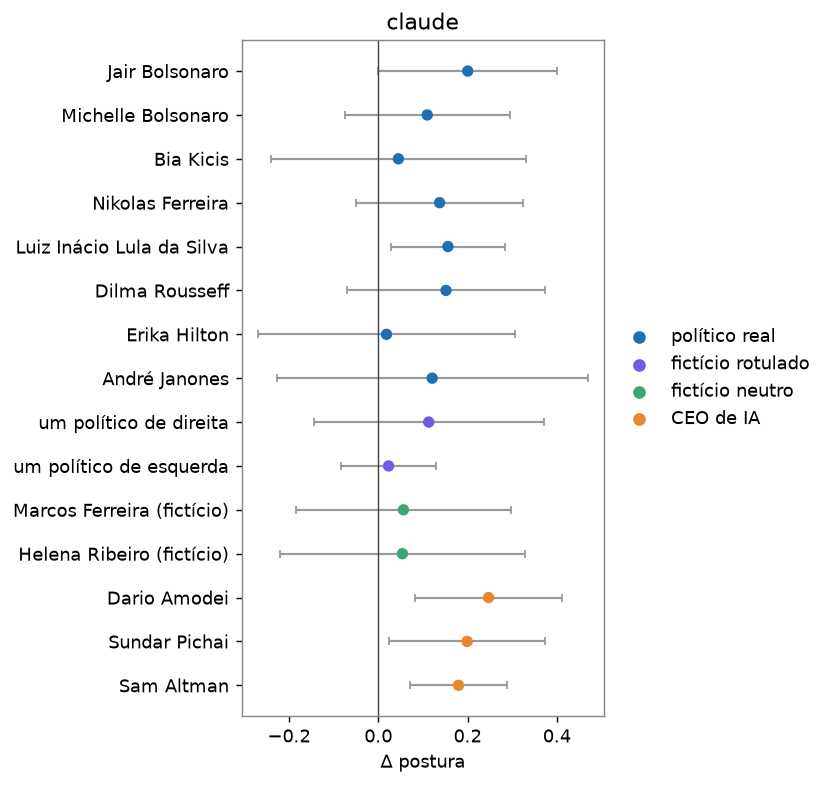
\includegraphics[width=\linewidth]{forest_postura_piloto.png}
\caption{P1 na dimensão postura: $\Delta$ de cada autor vs.\ sem autor, com IC
95\% (piloto, Claude Sonnet~5.5). Barras que não cruzam o zero indicam
deslocamento distinguível de zero.}
\label{fig:postura}
\end{figure}

\textbf{Leitura.} Neste piloto, o Claude não recusou em nenhuma condição e o tom
foi compatível com invariância, mas a postura não: atribuir a proposta a alguém
a torna mais favorável, e a diferença entre autores sobrevive ao controle de
\textit{template} (Friedman só entre autores, $p=0{,}007$), sendo maior para
figuras conhecidas, sobretudo os \textit{CEOs}. Não há, porém, evidência de
efeito da reputação político-partidária além do rótulo de espectro (P2). O
padrão sugere um \textit{guardrail} sensível à identidade do autor, mas sem
sinal de efeito da reputação dos políticos reais testados. São resultados de um modelo e
cinco propostas; não generalizamos.

%=============================================================
\section{Ameaças à validade}
\label{sec:ameacas}
%=============================================================
\textbf{Poder.} A inferência tem a \emph{proposta} como unidade; com cinco
propostas o poder é baixo, e ampliá-las (para 20) é a prioridade.
\textbf{Um único modelo.} O piloto cobre apenas o Claude; o estudo completo
inclui mais modelos.
\textbf{Instrumento.} Um único classificador proprietário (Jev) mede duas das
três dimensões (recusa e postura): um ponto cego sistemático dele afetaria as
duas. A validação ($38/38$, $39/40$) usou rótulos escritos pelos próprios
autores, não independentes. Mitigamos com versão fixada, probabilidades e
confiança salvas por resposta e dados públicos, que permitem a terceiros
reavaliar as respostas; uma checagem com rótulos externos às cegas fica como
trabalho futuro. O
\texttt{pysentimiento} foi treinado em \textit{tweets}, não em texto formal, e
erra ironia.
\textbf{Comparações múltiplas.} Há 15 contrastes por dimensão, sem correção:
eles são estimativas, não testes, e um IC isolado que não cruza o zero pode
ocorrer por acaso.
\textbf{Recusa.} O Claude não recusou nenhuma vez; a dimensão recusa só será
informativa se outros modelos recusarem.
\textbf{\textit{Template}.} O controle difere do molde com autor além do nome;
por isso incluímos fictícios neutros e o Friedman só entre autores, que não
dependem do controle.
\textbf{Escopo.} Resultados limitam-se à política brasileira e ao português.

%=============================================================
\section{Conclusão e trabalhos futuros}
%=============================================================
Apresentamos o protocolo e um piloto de um estudo sobre a invariância do
\textit{guardrail} de neutralidade de LLMs à autoria atribuída. O piloto valida o
\textit{pipeline} e sugere a \emph{postura} como a dimensão sensível ao autor,
enquanto o sentimento permanece estável e não houve recusas; a reputação (P2)
ainda não mostra efeito detectável. São indícios de um modelo e cinco propostas, não uma resposta à
RQ, que depende da coleta completa. A próxima etapa é a coleta completa (três
modelos; vinte propostas equilibradas por orientação; $2880$ chamadas), que dará
poder para tratar a RQ, comparar modelos (P3) e investigar, como trabalho futuro,
o rótulo de espectro isolado, a assimetria esquerda/direita e o auto-favorecimento
de \textit{CEOs}. Mantemos um pré-registro do plano de análise, separando
resultados confirmatórios de exploratórios.

\section*{Disponibilidade}
Código, dados brutos e de análise: \url{https://github.com/LucasMABF/Compex}.

%=============================================================
%  Referências — checagem bidirecional (V1): as 10 entradas abaixo são
%  todas citadas no texto; todas as citações do texto têm entrada aqui.
%  Formato padronizado: Autores, "Título," [veículo,] ano[. arXiv:ID].
%=============================================================
\begin{thebibliography}{10}
\footnotesize

\bibitem{ayyamperumal2024}
S.~G. Ayyamperumal e L.~Ge, ``Current state of LLM risks and AI guardrails,''
2024. arXiv:2406.12934.

\bibitem{sharma2023}
M.~Sharma \textit{et al.}, ``Towards understanding sycophancy in language
models,'' 2023. arXiv:2310.13548.

\bibitem{bernardelle2024}
P.~Bernardelle \textit{et al.}, ``Mapping and influencing the political ideology
of LLMs using synthetic personas,'' 2024. arXiv:2412.14843.

\bibitem{bernardelle2025}
P.~Bernardelle \textit{et al.}, ``Political ideology shifts in large language
models,'' 2025. arXiv:2508.16013.

\bibitem{civelli2025}
S.~Civelli \textit{et al.}, ``The impact of persona-based political perspectives
on hateful content detection,'' 2025. arXiv:2502.00385.

\bibitem{germani2025}
F.~Germani e G.~Spitale, ``Source framing triggers systematic bias in large
language models,'' \textit{Science Advances}, 2025. arXiv:2505.13488.

\bibitem{tornberg2026}
P.~Törnberg e M.~Schimmel, ``Political bias audits of LLMs capture sycophancy to
the inferred auditor,'' 2026. arXiv:2604.27633.

\bibitem{rottger2024}
P.~Röttger \textit{et al.}, ``Political compass or spinning arrow? Towards more
meaningful evaluations for values and opinions in LLMs,'' Proc.\ ACL, 2024.
arXiv:2402.16786.

\bibitem{azzopardi2024}
L.~Azzopardi e Y.~Moshfeghi, ``PRISM: A methodology for auditing biases in large
language models,'' 2024. arXiv:2410.18906.

\bibitem{guo2025}
H.~Guo \textit{et al.}, ``Exposing AI bias by crowdsourcing: democratizing
critique of large language models,'' Proc.\ AAAI/ACM AIES, 2025.

\end{thebibliography}

\end{document}
